\begin{flushleft}
{\Huge Hyfsvisor\\}
\vspace{1 cm}
{\Large
När huvudrätten lider mot sitt slut och gästerna är mätta och belåtna
kungör toastmastern hyfs. Vid hyfs sjunges en av
hyfsvisorna nedan, varpå all vätska i glasen drickes upp. Detta sker för att bereda plats för punsch eller dylik söt dryck till
efterrätten. Efter hyfsandet serveras efterrätten med kaffe och avec.}
\end{flushleft}

\vspace{2cm}
\begin{center}
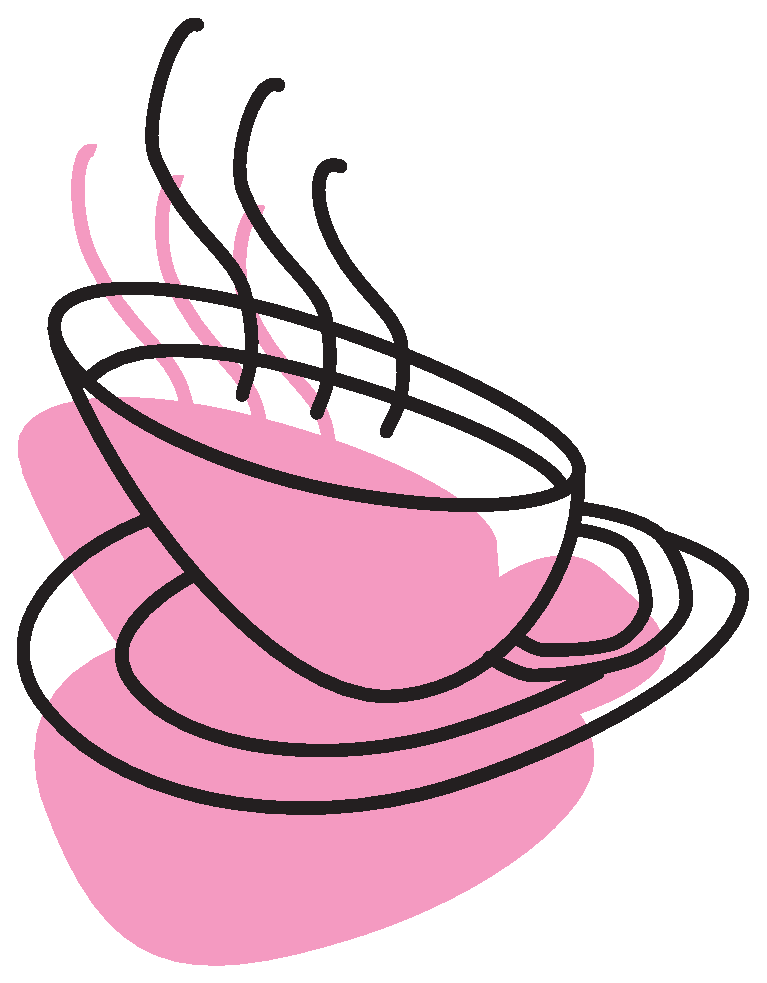
\includegraphics[width=6cm]{bilder/43.eps}
\end{center}
\newpage

\inputsong{harjarevisan}

\inputsong{kalmarevisan}









